\chapter{听觉fMRI数据}

该实验由 Geraint Rees 在 Karl Friston 和 FIL 方法组的指导下进行。 目的是在我们早期的 fMRI 体验中探索设备和技术。 因此,它尚未正式编写,可免费用于个人教育和评估目的。

该数据集是功能成像实验室 (FIL) 首次收集和分析的数据集,在当地被称为所有实验之母 (MoAE)。

该数据集包含在改进的 2T Siemens MAGNETOM Vision 系统上获取的全脑 BOLD/EPI 图像。 每次采集都包含 64 个连续切片(64 $\times$ 64 $\times$ 64 $\times$ 3 $\times$ 3 $\times$ 3 mm3 体素)。 采集耗时 6.05 秒,扫描重复时间 (TR) 任意设置为 7 秒。

从单个对象进行了 96 次采集(TR = 7s),以 6 个为一组,给出 16 个 42s 块。 从休息开始,连续块的条件在休息和听觉刺激之间交替。 听觉刺激是以每分钟 60 次的速度双耳呈现的双音节词。 功能数据从采集 4 开始,图像 fM00223\_004.{hdr,img},并存储在文件夹 fM00223 中。 由于 T1 效应,建议放弃前几次扫描(没有“虚拟”导入扫描)。 还获取了结构图像:sM00223\_002.{hdr,img},存储在文件夹 sM00223 中。 这些图像以 Analyze 格式存储(现在已被 NIfTI 格式取代,但 SPM 可以本地读取这两种格式并始终将图像保存为 NIfTI)并且可以从 SPM 站点获得\footnote{fMRI听觉数据集: http://www.fil.ion.ucl.ac.uk/spm/data/auditory/}。

要分析数据,首先创建一个新目录 DIR,例如。 C:ndatanauditory,其中放置您的分析结果。 然后创建 3 个子目录 (i) dummy,(ii) jobs 和 (iii) classical。 随着分析的进行,这些目录将充满虚拟扫描、作业规范文件、设计矩阵和使用经典推理估计的模型。

启动 Matlab 进入您的作业目录并在 Matlab 提示符下键入 spm fmri。 然后 SPM 将在 fMRI 模式下打开三个窗口(参见图\ref{fig_30_1}):(1) 左上角或“菜单”窗口,(2) 左下角或“交互”窗口和 (3) 右手或 “图形”窗口。 然后在三个主要阶段进行分析 (i) 空间预处理,(ii) 模型规范、审查和估计以及 (iii) 推理。 这些阶段组织了 SPM 菜单窗口中的按钮。

\begin{figure}[htbp]
	\centering
	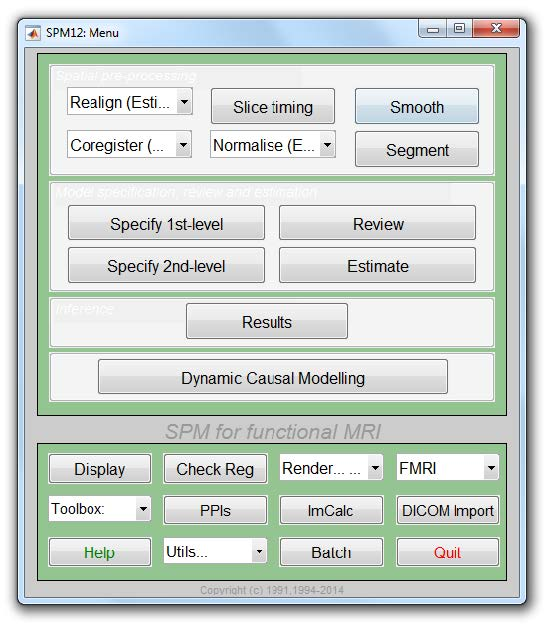
\includegraphics[width=0.6\linewidth]{part7/figs/fig_30_1}
	\caption{SPM 基本窗口包括三个部分 (i) 空间预处理,(ii) 模型规范、审查和估计以及 (iii) 推理。}
	\label{fig_30_1}
\end{figure}

\section{序言(dummy scans)}
为了避免在 fMRI 时间序列的初始扫描中产生 T1 效应,我们建议丢弃前几次扫描。 为了简化这个例子,我们将丢弃第一个完整的循环(12 次扫描,04-15),留下 84 次扫描,图像文件 16-99。 最好通过将这些文件移动到我们之前创建的不同目录 dummy 来完成。


\section{空间预处理}

\subsection{头动校正}
在 SPM 菜单窗口的空间预处理部分下,从重新对齐下拉菜单中选择重新对齐(Est \& Res)。 这将在批处理编辑器中调用重新对齐作业规范。 然后

\begin{itemize}
	\item 突出显示“Data”,选择“New Session”,然后突出显示新创建的“Session”选项。
	
	\item 按“选择文件”并使用 SPM 文件选择器选择所有功能图像,例如。 (“fM000*.img”)。 应该有84个文件。
	
	\item 按“Reslice Options”中的“Resliced images”并选择“Mean Image Only”。
	
	\item 将作业文件保存为例如。 DIR\\jobs\\realign.mat。
	
	\item 按批处理编辑器中的运行按钮(绿色箭头)。
\end{itemize}


这将运行 realign 作业,它将估计 6 参数(刚体)空间变换,它将对齐图像的时间序列,并将修改输入图像 (*.hdr) 的标题,以便它们反映图像的相对方向 校正运动伪影后的数据。 然后 SPM 将绘制图 30.2 中所示的平移和旋转的估计时间序列。 这些数据也被保存到一个文件中,例如。 rp\_fM00223\_016.txt,以便以后在拟合 GLM 时可以将这些变量用作回归量。 这允许在寻找大脑激活时打折运动效果。

SPM 还将创建平均图像,例如。 meanfM00223\_016.img 将用于下一步的空间处理 - 配准。

\begin{figure}[htbp]
	\centering
	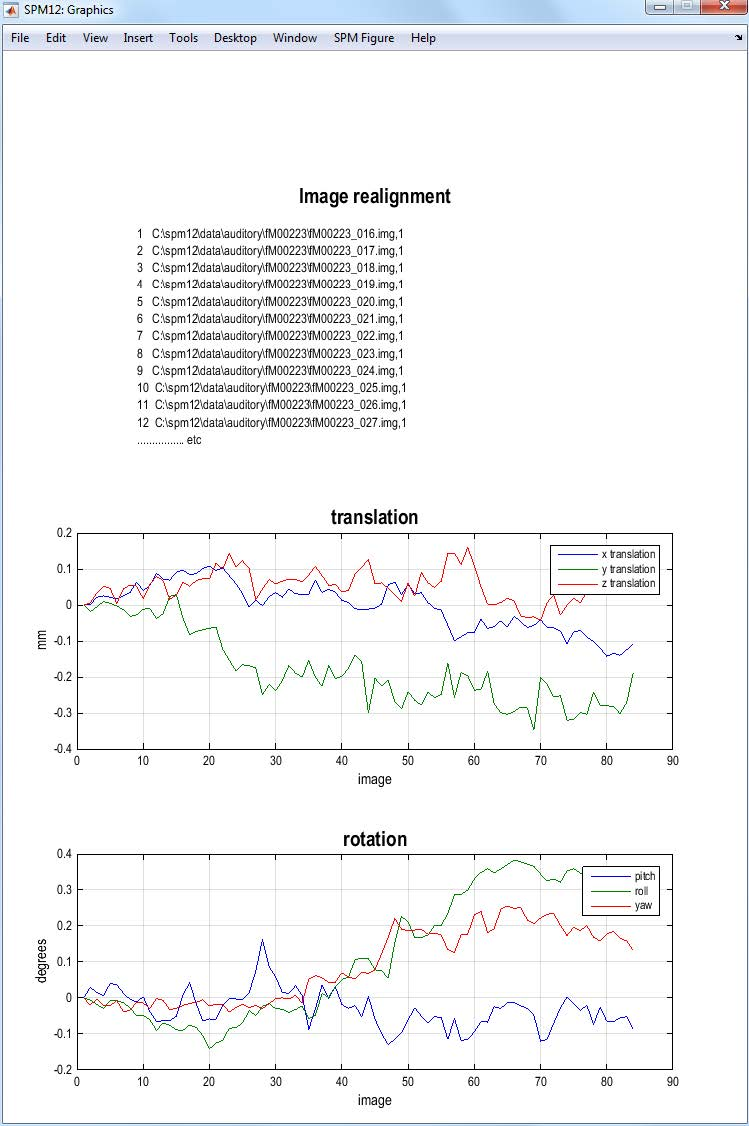
\includegraphics[width=0.6\linewidth]{part7/figs/fig_30_2}
	\caption{听觉数据的头动校正}
	\label{realignment}
\end{figure}

\subsection{配准}

从 Coregister 下拉菜单中选择 Coregister (Estimate)。 这将在批处理编辑器中调用配准作业的规范。

\begin{itemize}
	\item 突出显示“参考图像”,然后从重新对齐中选择平均 fMRI 扫描,例如。 meanfM00223\_016.img。
	
	\item 突出显示“源图像”,然后选择结构图像,例如。 sM00223\_002.img。
	
	\item 按保存按钮并将作业保存为 DIR\\jobs\\coregister.mat。
	
	\item 然后按下运行按钮。
\end{itemize}


然后,SPM 将在结构数据和功能数据之间实施配准,以最大化互信息。 然后图 30.3 中的图像应该出现在图形窗口中。 SPM 将更改源文件的标头,在本例中为结构图像 sM00223\_002.hdr。

Check Reg 工具在这里很有用,可以检查配准的结果。 按菜单窗口下部的检查注册按钮,然后选择上面指定的“参考”和“源”图像,即 meanfM00223\_016.img 和 sM00223\_002.img。 然后 SPM 将在图形窗口中生成如图 30.4 所示的图像。 然后,您可以使用鼠标浏览这些图像以确认存在解剖对应关系。

\begin{figure}[htbp]
	\centering
	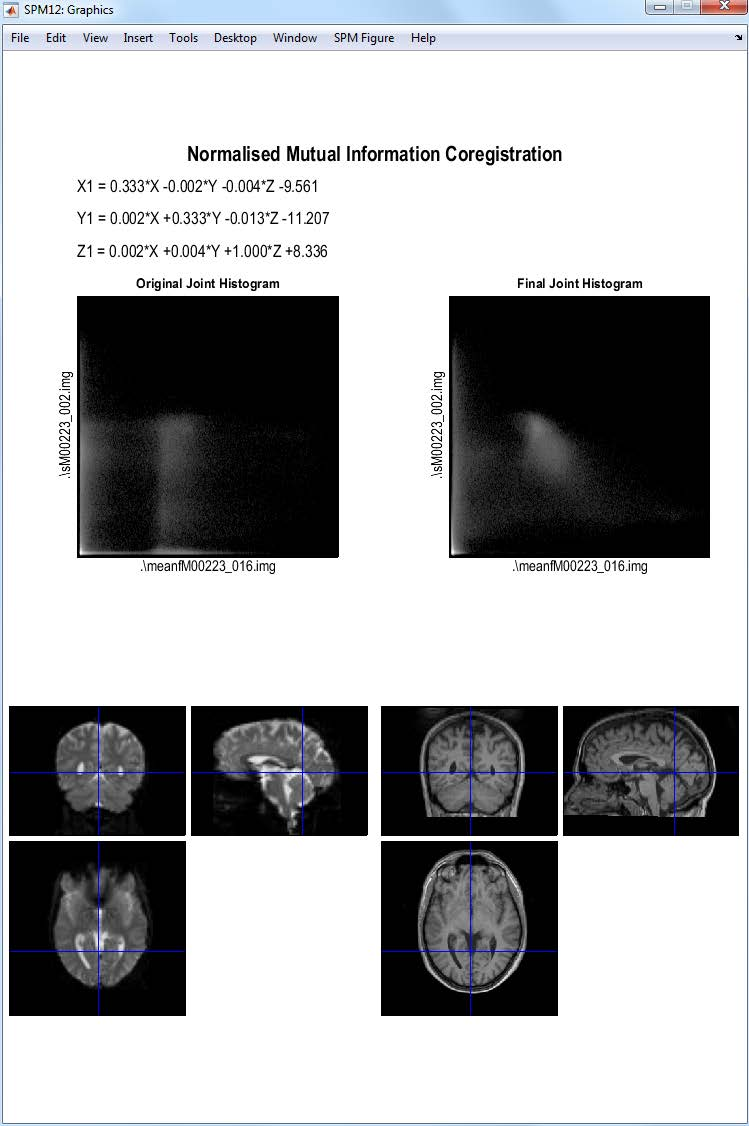
\includegraphics[width=0.6\linewidth]{part7/figs/fig_30_3}
	\caption{听觉数据的互信息配准。}
	\label{mutual_information}
\end{figure}

\begin{figure}[htbp]
	\centering
	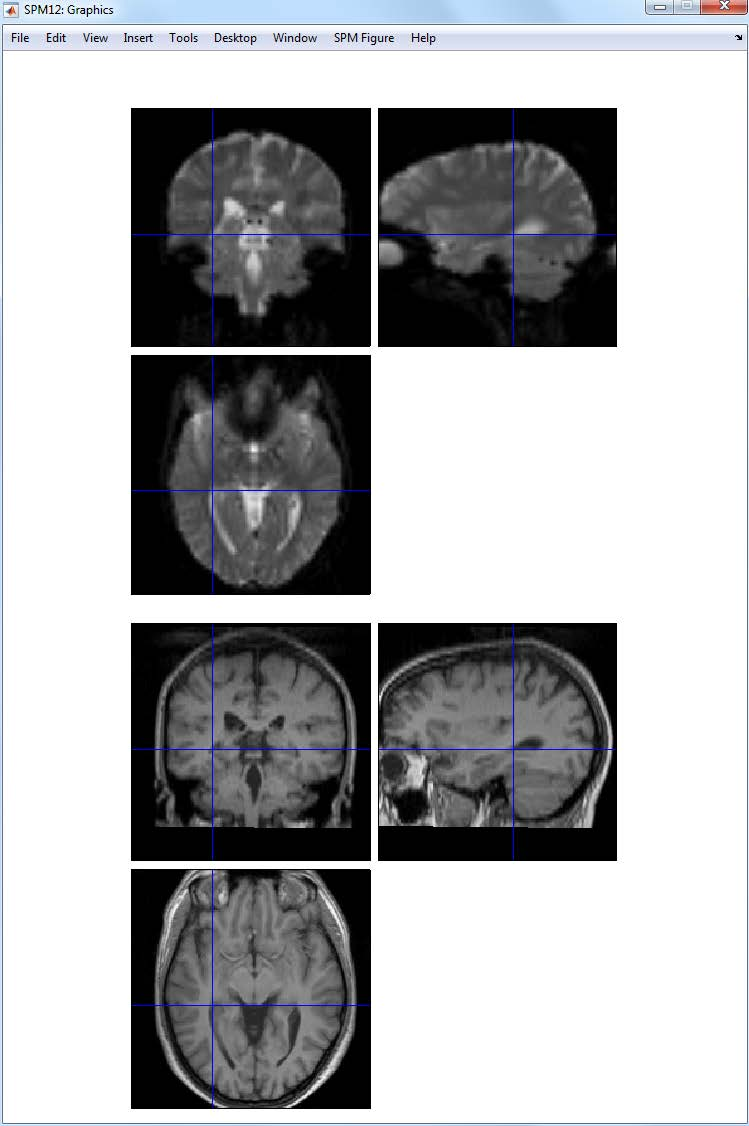
\includegraphics[width=0.6\linewidth]{part7/figs/fig_30_4}
	\caption{检查功能和“已注册”结构数据的注册。}
	\label{checking_registration}
\end{figure}

\subsection{分割}
按分段按钮。 这将在批处理编辑器中调用分段作业的规范。 突出显示“卷”字段,然后选择主题的注册解剖图像,例如。 sM00223\_002.img。 突出显示“Save Bias Corrected”并选择“Save Bias Corrected”。 突出显示列表底部的“变形场”并选择“向前”。 将作业文件另存为 segment.mat,然后按运行。 SPM 将使用默认的组织概率图作为先验 [9] 来分割结构图像。

SPM 将创建灰质和白质图像以及偏置场校正结构图像。 这些可以使用 CheckReg 工具查看,如上一节所述。 图 30.5 显示了灰质图像 c1sM0023\_002.nii 以及原始结构。 图 30.6 显示了结构和偏差校正图像,msM0023\_002.nii。

SPM 还会在原始结构目录中写入一个变形场,文件 y\_sM00223\_002.nii。 它包含 3 个卷来编码 x、y 和 z 坐标。 鉴于结构和功能数据对齐,这可用于空间归一化功能数据。

\subsection{正则化}
从 Normalize 下拉菜单中选择 Normalize (Write)。 这将在批处理编辑器中调用规范化作业的规范。

\begin{itemize}
	\item 突出显示“数据”,选择新建“主题”,
	
	\item 突出显示“变形场”并选择您在上一节中创建的 y\_sM00223\_002.nii 文件,
	
	\item 突出显示“要写入的图像”并选择所有重新对齐的功能图像 fM000*.img。 您可以右键单击列出的文件,选择“全选”,然后按“完成”。
	
	\item 在“书写选项”中,将“体素大小”从 [2 2 2] 更改为 [3 3 3]。 此步骤并非绝对必要:它会以更接近获取图像时的分辨率写出图像。
	
	\item 按“保存”,将作业保存为 normalise\_functional.mat,然后按“运行”按钮。
\end{itemize}

SPM 然后将空间归一化文件写入功能数据目录。 这些文件有前缀 w。

如果您希望将受试者的功能激活叠加在他们自己的解剖结构上,您还需要将空间归一化参数应用于他们的(偏差校正)解剖图像。 去做这个

\begin{itemize}
	\item 选择标准化(写入),突出显示“数据”,选择“新主题”。
	
	\item 突出显示“变形场”,选择您在上一节中创建的 y\_sM00223\_002.nii 文件,按“完成”。
	
	\item 突出显示“要写入的图像”,选择偏差校正结构,例如。 msM00223\_002.nii,按“完成”。
	
	\item 打开“Writing Options”,选择体素大小,将默认的[2 2 2]更改为[1 1 3],对应于图像的原始分辨率。
	
	\item 将作业另存为 normalise\_structural.mat 并按下 RUN 按钮。
\end{itemize}



\subsection{平滑}
按平滑按钮。 这将在批处理编辑器中调用平滑作业的规范。

\begin{itemize}
	\item 选择“要平滑的图像”,然后选择在上一节中创建的空间归一化文件,例如。 wf*.img。 这可以通过将 SPM 文件选择器中的过滤器更改为 \^wf.* 来有效地完成。 SPM 将只列出那些以字母 wf 开头的文件。 那些已经空间标准化的。
	
	\item 突出显示“FWHM”并将 [8 8 8] 更改为 [6 6 6]。 这将在每个方向上将数据平滑 6mm。
	
	\item 将作业另存为 smooth.mat 并按下运行按钮。
	
	\item 图 30.7 显示了功能图像及其平滑版本的示例。
\end{itemize}


\begin{figure}[htbp]
	\centering
	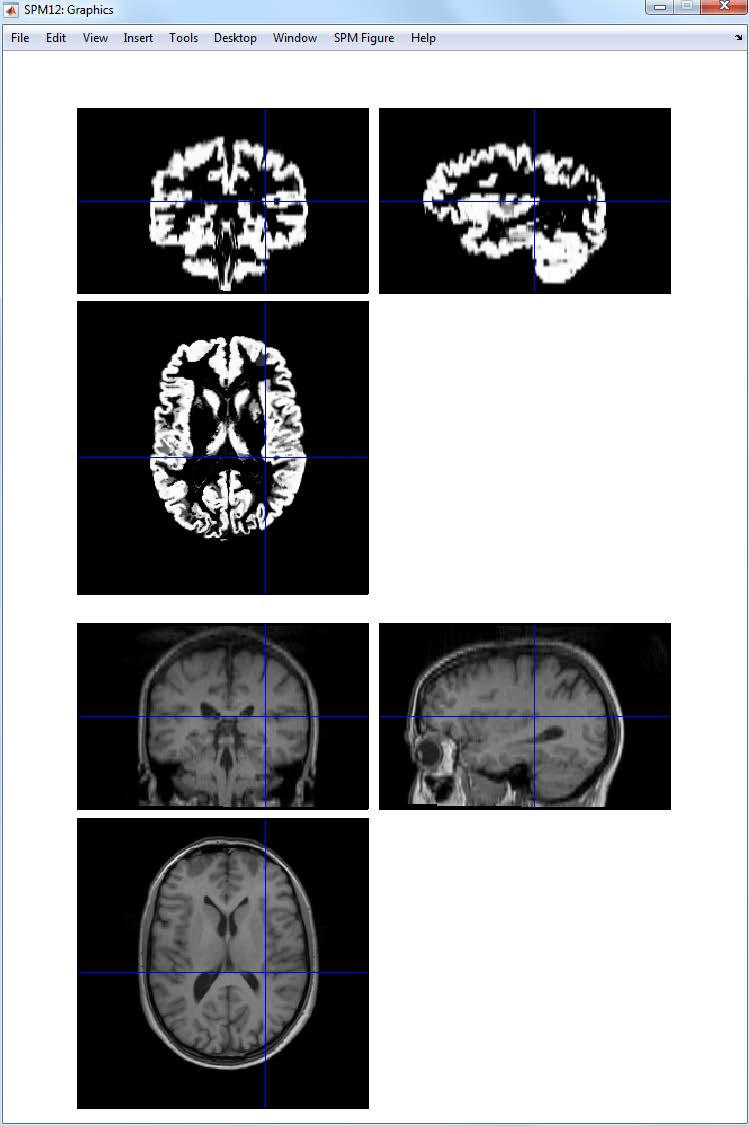
\includegraphics[width=0.6\linewidth]{part7/figs/fig_30_5}
	\caption{听觉数据的头动校正}
	\label{gray_matter}
\end{figure}


\begin{figure}[htbp]
	\centering
	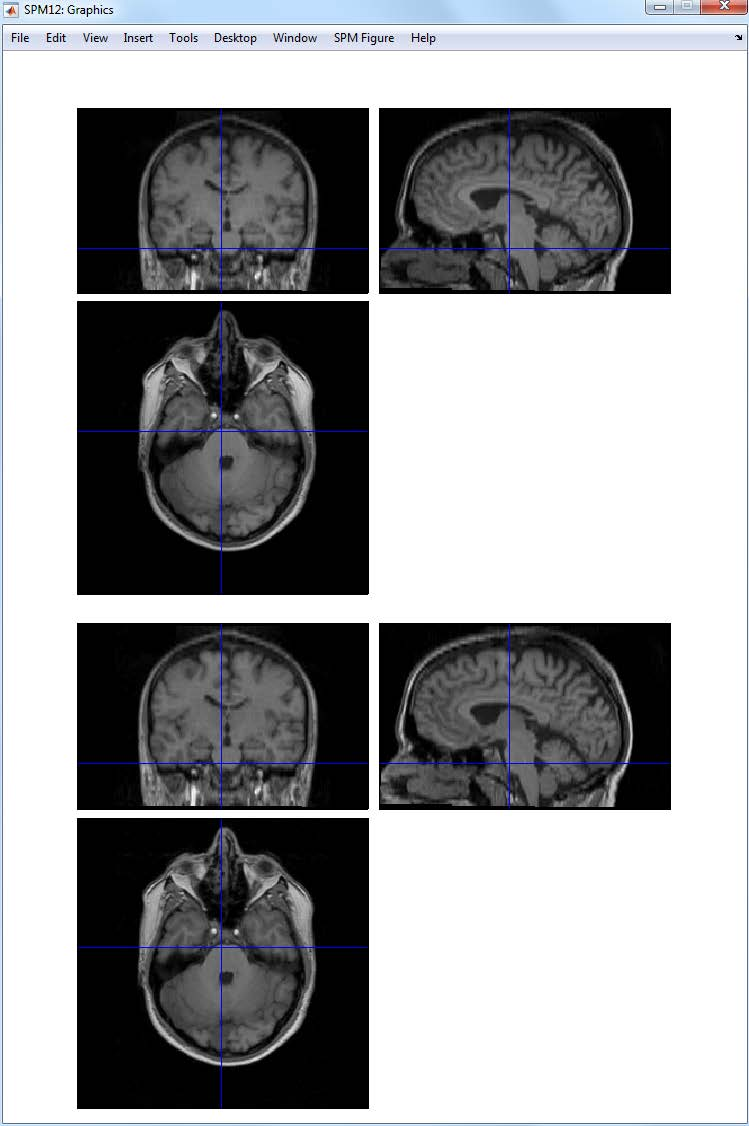
\includegraphics[width=0.6\linewidth]{part7/figs/fig_30_6}
	\caption{结构图像(顶部)和偏差校正结构图像(底部)。 请注意,原始结构在顶部比底部更暗。 这种不均匀性已在偏差校正图像中消除。}
	\label{structural_image}
\end{figure}

\begin{figure}[htbp]
	\centering
	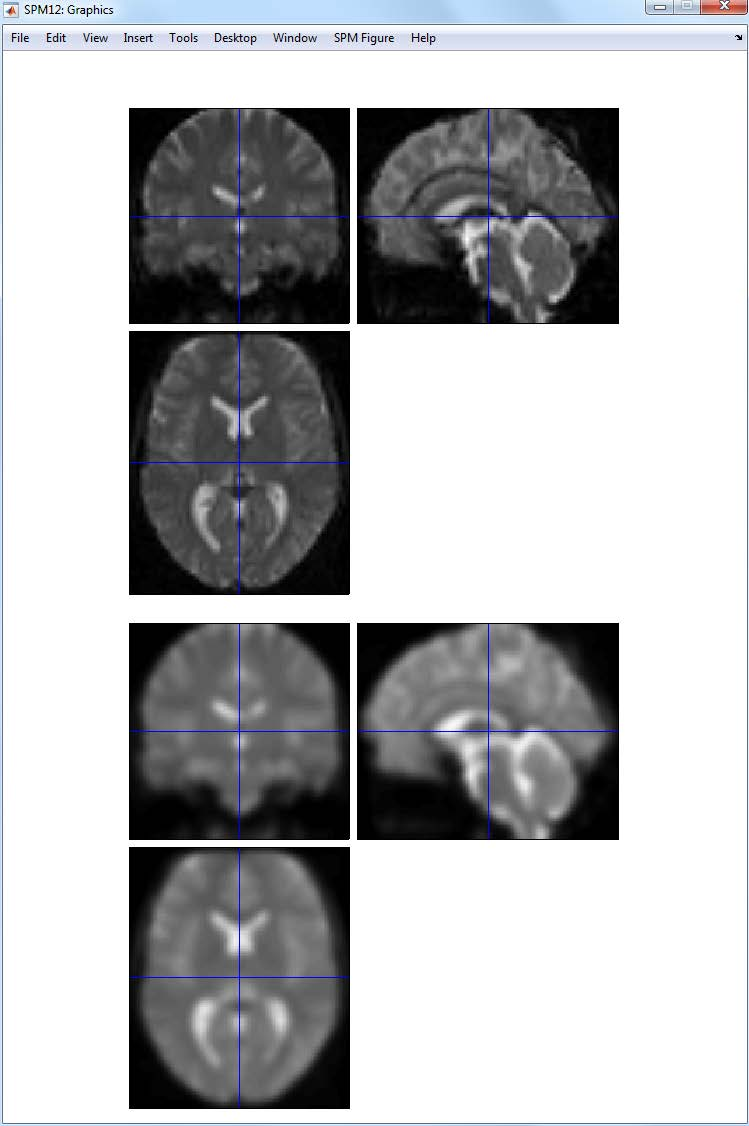
\includegraphics[width=0.6\linewidth]{part7/figs/fig_30_7}
	\caption{结构图像(顶部)和偏差校正结构图像(底部)。 请注意,原始结构在顶部比底部更暗。 这种不均匀性已在偏差校正图像中消除。}
	\label{functional_image}
\end{figure}


\section{模型定义、检查和估计}

按“指定第一级”按钮。 这将在批处理编辑器中调用 fMRI 规范作业的规范。 然后
\begin{itemize}
	\item 打开“时序参数”选项。
	\item 突出显示“设计单位”并选择“扫描”。
	\item 突出显示“Interscan interval”并输入 7。这是以秒为单位的 TR。
	\item 突出显示“数据和设计”并选择“新主题/会话”。 然后打开新创建的“Subject/Session”选项。
	\item 突出显示“扫描”并使用 SPM 的文件选择器选择 84 个平滑、标准化的功能图像,即 swfM00223\_016.img 到 swfM00223\_099.img。 这些可以使用 \^sw.*' 过滤器轻松选择,然后全选。 然后按“完成”。
	\item 突出显示“条件”并选择“新条件”。
	\item 打开新创建的“条件”选项。 突出显示“名称”并输入“收听”。 突出显示“起始”并输入“6:12:84”。 突出显示“持续时间”并输入“6”。
	\item 突出显示“目录”并选择您之前创建的 DIR/classical 目录。
	\item 将作业另存为 specify.mat 并按下运行按钮。
\end{itemize}

SPM 然后会将 SPM.mat 文件写入 DIR/classical 目录。 它还将绘制设计矩阵,如图 30.8 所示。

在此阶段,建议使用 SPM 的审查工具检查您的模型规格,该工具可通过“审查”按钮访问。 这会在交互式窗口中弹出一个“设计”选项卡,单击它会产生一个下拉菜单。 如果您选择第一项“Design Matrix”,SPM 将生成如图 30.8 所示的图像。 如果您选择“Explore”,然后选择“Session 1”,然后选择“listening”,SPM 将生成如图 30.9 所示的图。

如果您选择“设计”选项卡上的第二项“设计正交性”,SPM 将生成如图 30.10 所示的图。 如果内积 xT1 x2 = 0,则 x1 和 x2 列是正交的。内积也可以写成 xT1 x2 = jx1jjx2jcos,其中 jxj 表示 x 的长度,是两个向量之间的角度。 因此,如果 cos = 0,向量将是正交的。图 30.10 底部矩阵中的上对角线元素绘制了设计矩阵中每对列的 cos。 这里我们有一个条目。 灰色阴影表示一定程度的非正交性或共线性。

\subsection{估计}
按估计按钮。 这将在批处理编辑器中调用 fMRI 估计作业的规范。 然后

\begin{itemize}
	\item 突出显示“选择 SPM.mat”选项,然后选择保存在经典子目录中的 SPM.mat 文件。
	\item 将作业另存为 estimate.mat 并按下运行按钮。
\end{itemize}

SPM 会将许多文件写入所选目录,包括 SPM.mat 文件。




\section{推断}

估计之后:
\begin{itemize}
	\item 按“结果”。
	\item 选择在上一节中创建的 SPM.mat 文件。
\end{itemize}

这将调用对比度管理器。

\begin{figure}[htbp]
	\centering
	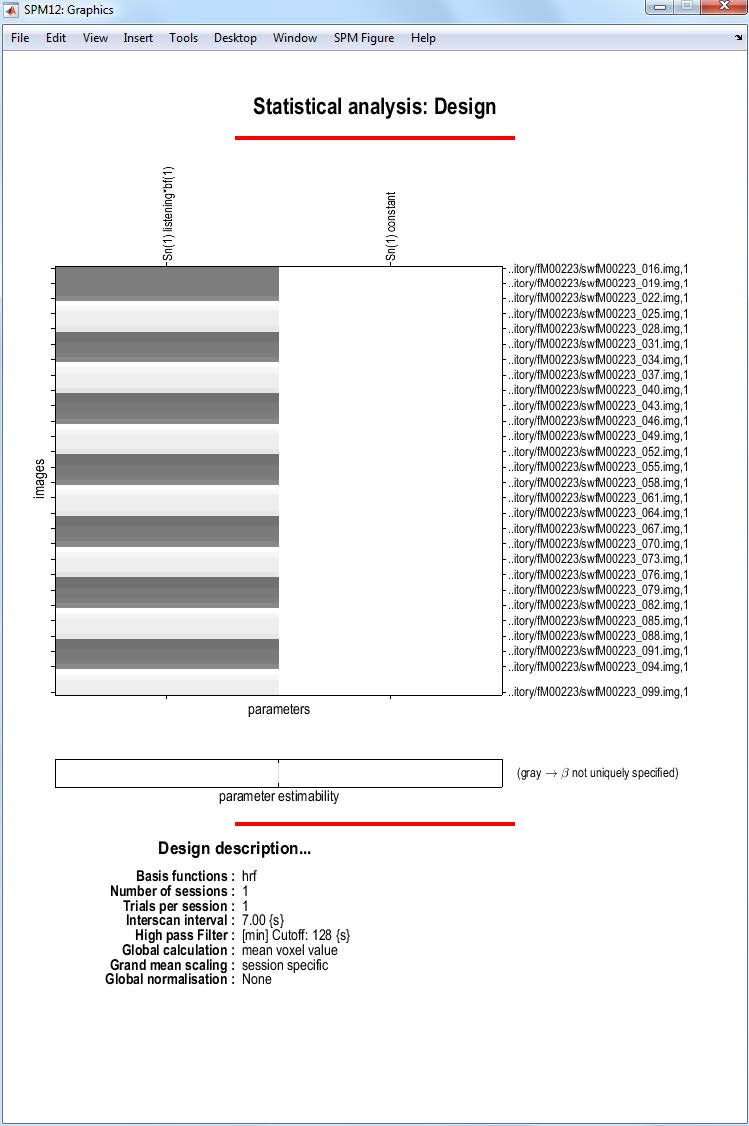
\includegraphics[width=0.6\linewidth]{part7/figs/fig_30_8}
	\caption{设计矩阵右侧的文件名表示与每一行关联的扫描。}
	\label{design_matrix}
\end{figure}

\begin{figure}[htbp]
	\centering
	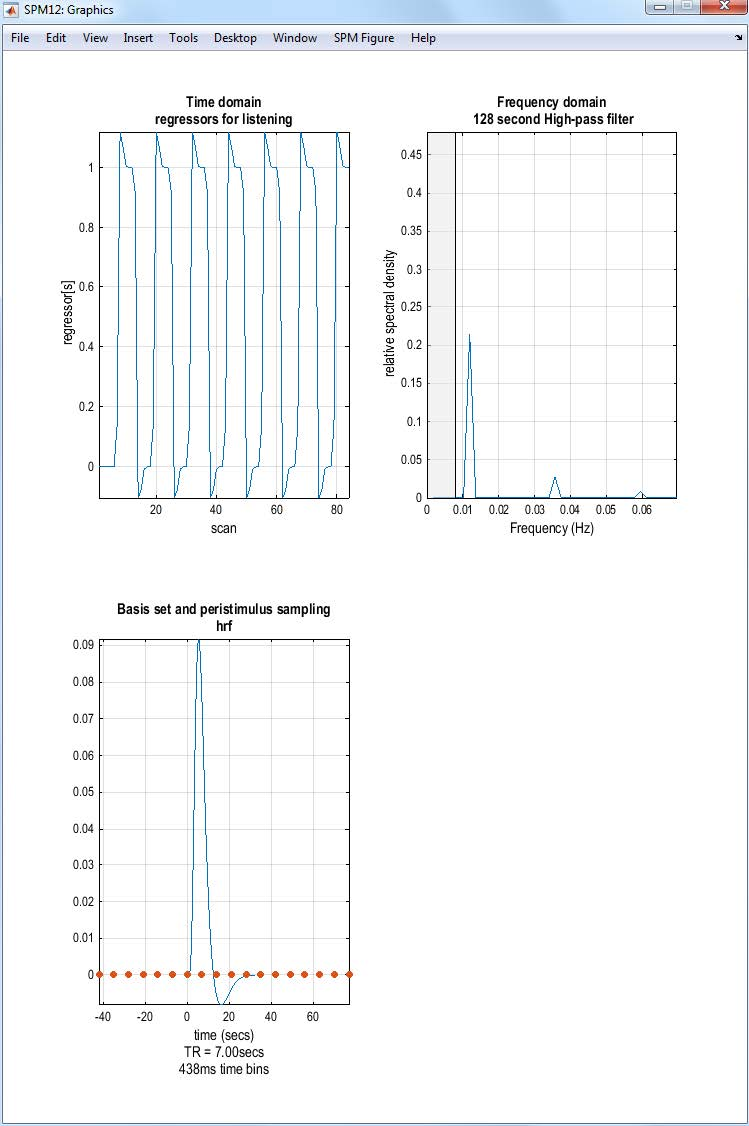
\includegraphics[width=0.6\linewidth]{part7/figs/fig_30_9}
	\caption{探索图 30.8 中的设计矩阵:这显示了“听”回归量的时间序列(左上)、“听”回归量的频域图(右上)和用于将假设的神经元活动转换为血液动力学的基函数 活动。 在这个模型中,我们使用了默认选项——规范基函数。 频域图显示“监听”回归器的频率内容高于被高通滤波器 (HPF) 移除的设定频率(这些以灰色显示 - 在该模型中我们接受了默认的 HPF 截止值 128 秒或 0.008Hz)。}
	\label{fig_30_9}
\end{figure}

\begin{figure}[htbp]
	\centering
	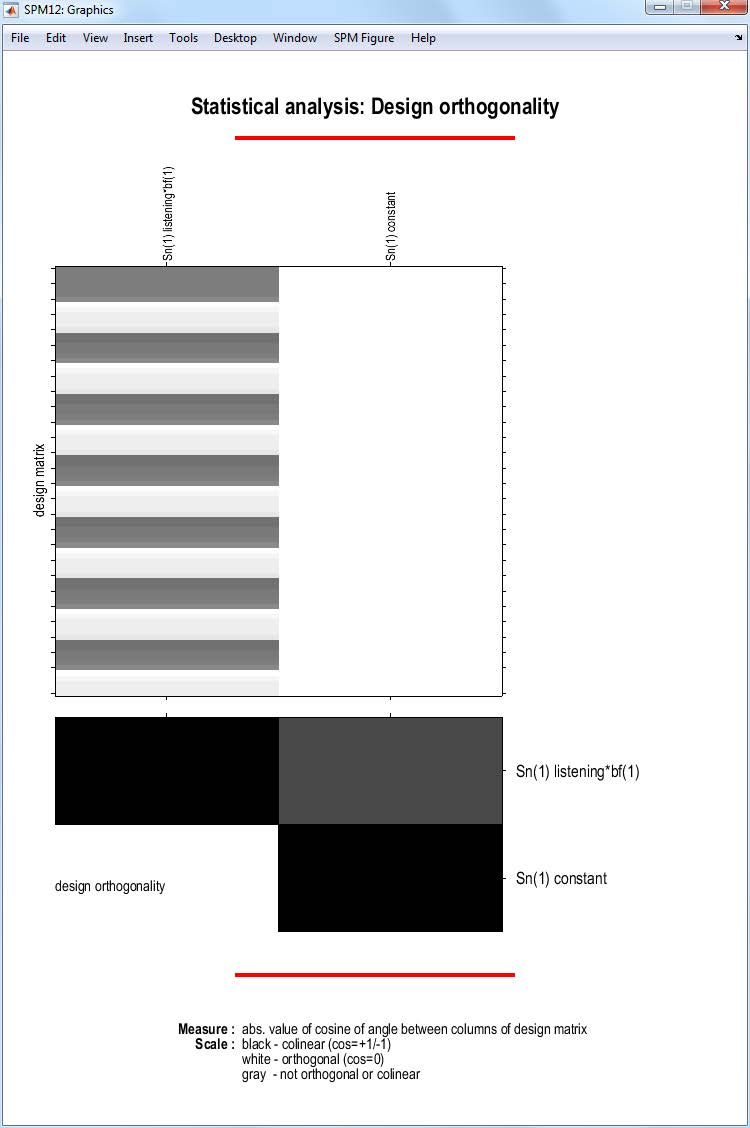
\includegraphics[width=0.6\linewidth]{part7/figs/fig_30_10}
	\caption{Design Orthogonality:设计矩阵Sn(1)Listening*bf(1)第一列上面的描述表示这一列指的是第一个session的数据(在这个分析中只有1个session),这个条件的名称 /trial 是'listening'并且试验信息已经与第一个基函数(典型的血液动力学响应)卷积。 会话 1 的常量回归量称为 Sn(1)Constant。 底部的正交矩阵表示回归变量之间的共线性程度。}
	\label{fig_30_10}
\end{figure}


\begin{figure}[htbp]
	\centering
	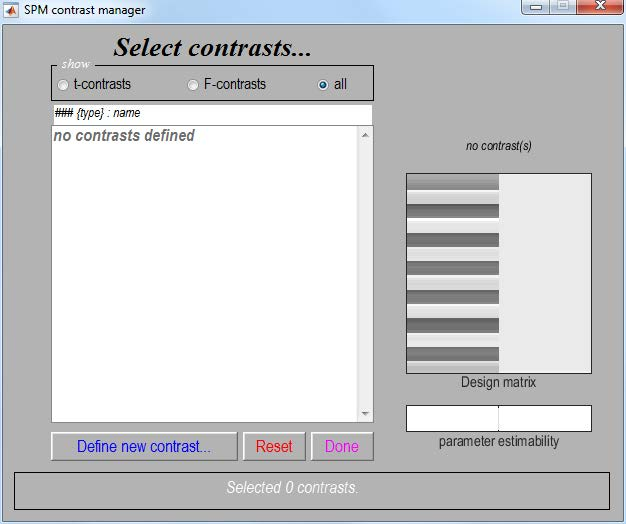
\includegraphics[width=0.6\linewidth]{part7/figs/fig_30_11}
	\caption{对比管理器}
	\label{fig_30_11}
\end{figure}

\begin{figure}[htbp]
	\centering
	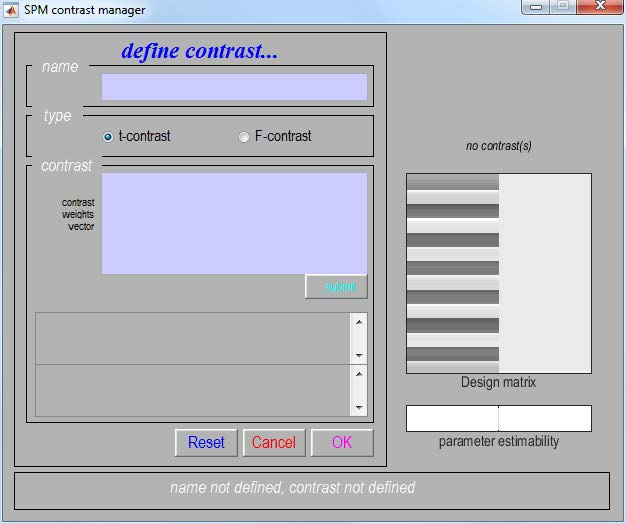
\includegraphics[width=0.6\linewidth]{part7/figs/fig_30_12}
	\caption{左图:通过在下部窗口中指定数值并在上部窗口中指定名称来输入对比度。 右:指定对比度后可以选择它们。}
	\label{fig_30_12}
\end{figure}

\begin{figure}[htbp]
	\centering
	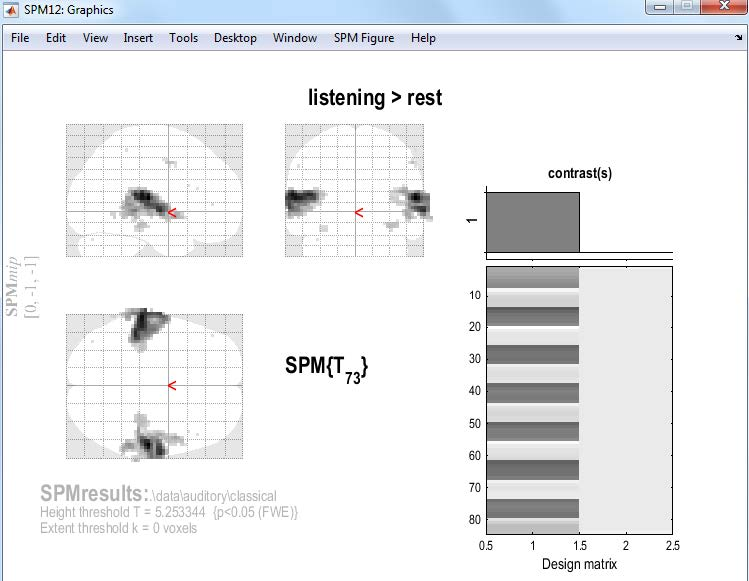
\includegraphics[width=0.6\linewidth]{part7/figs/fig_30_13}
	\caption{SPM 显示听觉皮层的双侧激活。}
	\label{fig_30_13}
\end{figure}

\begin{figure}[htbp]
	\centering
	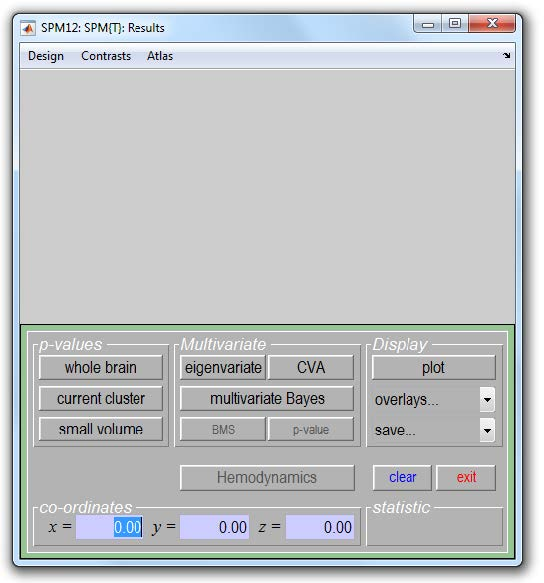
\includegraphics[width=0.6\linewidth]{part7/figs/fig_30_14}
	\caption{结果评估期间 SPM 的交互窗口。 “p 值”部分用于生成统计信息表。 可视化部分用于绘制体素响应或覆盖在解剖图像上的视觉激活。 “多变量”部分,即。 “本征变量”按钮用于提取数据用于后续分析,例如心理生理相互作用 (PPI) 或动态因果模型 (DCM) 的评估。}
	\label{fig_30_14}
\end{figure}

\begin{figure}[htbp]
	\centering
	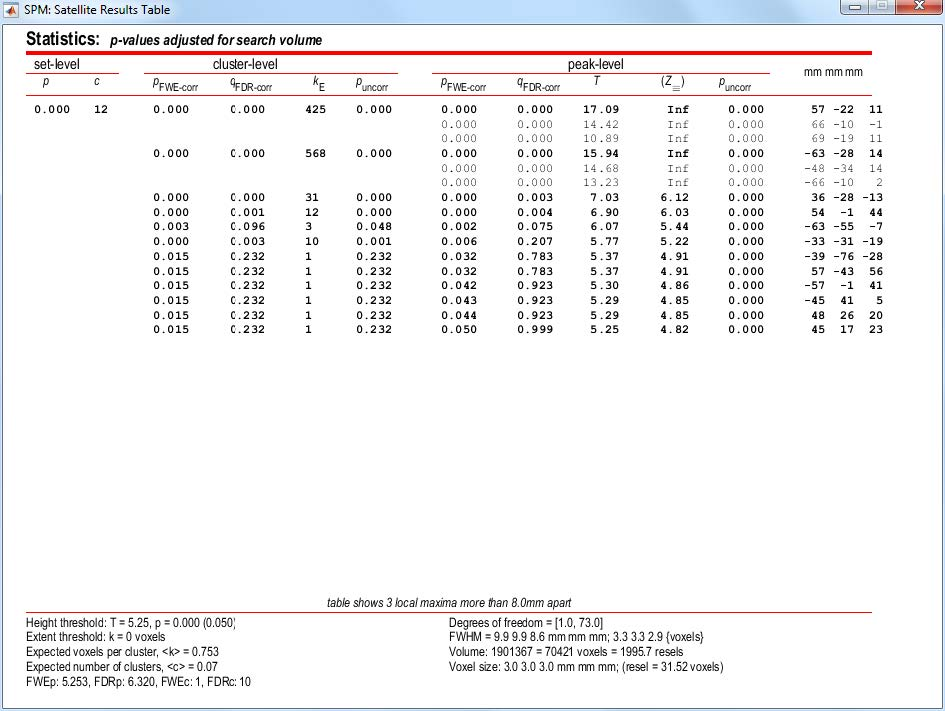
\includegraphics[width=0.6\linewidth]{part7/figs/fig_30_15}
	\caption{“聆听 > 休息”效果的音量表。 此值表是通过按“图形”窗口顶部的“SPM 图”>“结果表”选项,然后按“全脑”按钮创建的。 这会在单独的窗口中显示结果表。}
	\label{fig_30_15}
\end{figure}

\begin{figure}[htbp]
	\centering
	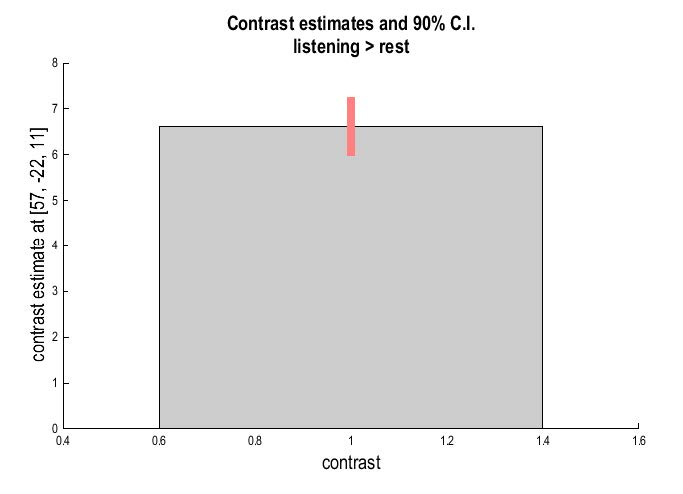
\includegraphics[width=0.6\linewidth]{part7/figs/fig_30_16}
	\caption{估计效应大小。}
	\label{fig_30_16}
\end{figure}

\begin{figure}[htbp]
	\centering
	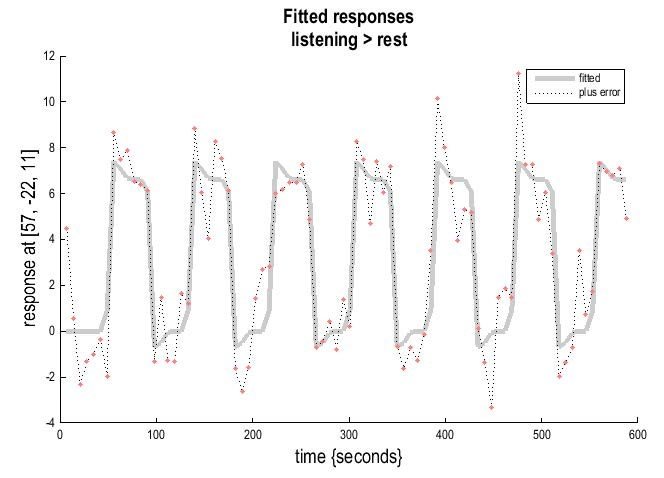
\includegraphics[width=0.6\linewidth]{part7/figs/fig_30_17}
	\caption{拟合响应。}
	\label{fig_30_17}
\end{figure}

\begin{figure}[htbp]
	\centering
	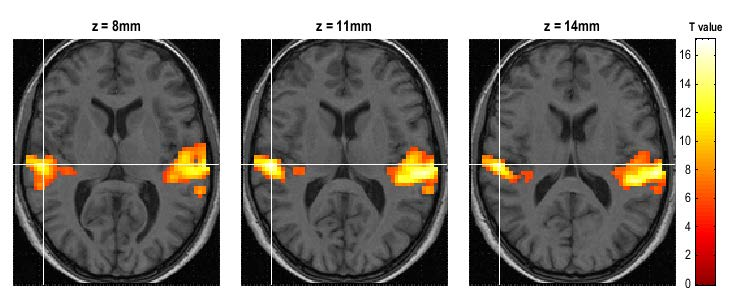
\includegraphics[width=0.6\linewidth]{part7/figs/fig_30_18}
	\caption{切片。}
	\label{fig_30_18}
\end{figure}

\begin{figure}[htbp]
	\centering
	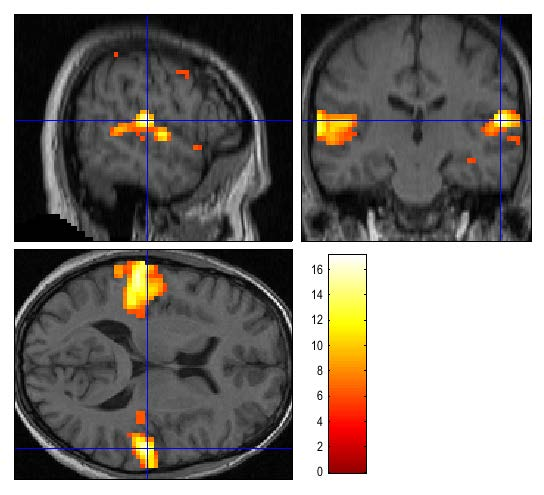
\includegraphics[width=0.6\linewidth]{part7/figs/fig_30_19}
	\caption{切片。}
	\label{fig_30_19}
\end{figure}

\begin{figure}[htbp]
	\centering
	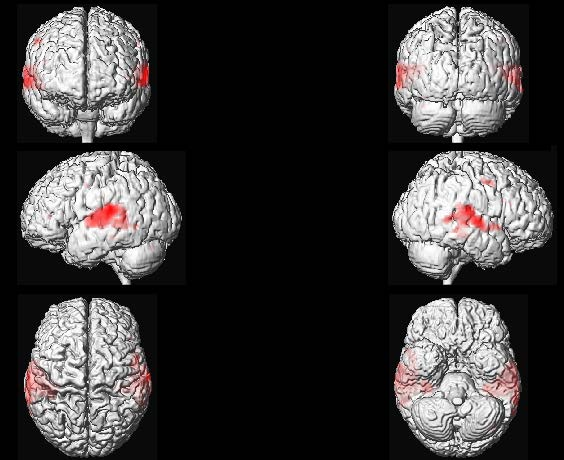
\includegraphics[width=0.6\linewidth]{part7/figs/fig_30_20}
	\caption{渲染。}
	\label{fig_30_20}
\end{figure}

\begin{figure}[htbp]
	\centering
	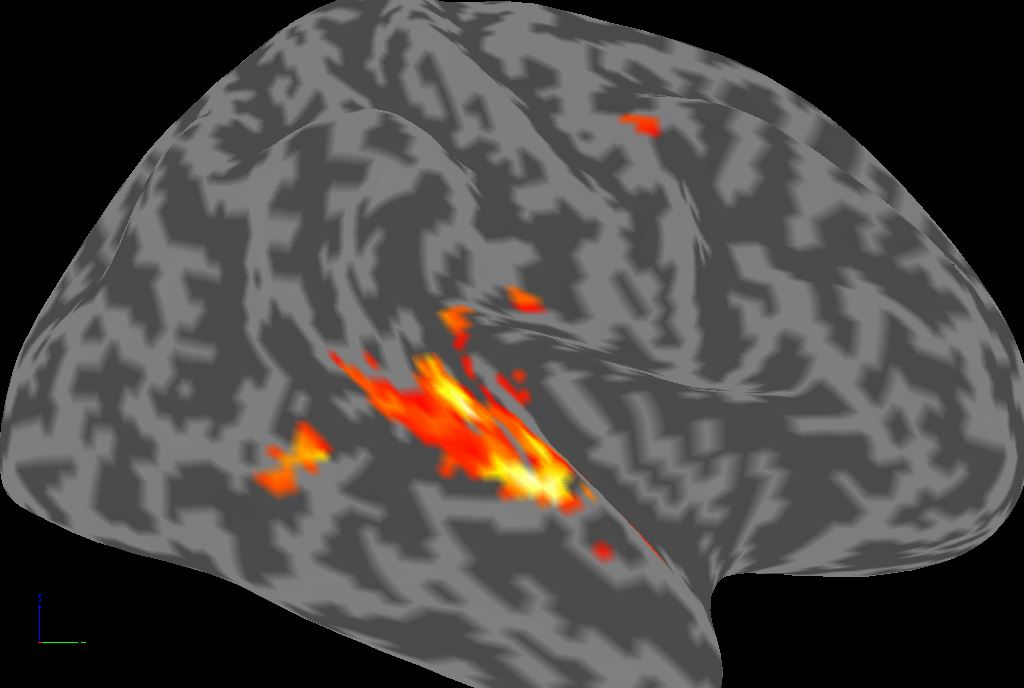
\includegraphics[width=0.6\linewidth]{part7/figs/fig_30_21}
	\caption{使用标准网格的 3D 渲染。}
	\label{fig_30_21}
\end{figure}


\subsection{对比管理器}
对比度管理器在右侧面板中显示设计矩阵(可浏览),并在左侧面板中列出指定的对比度。 可以选择“t-contrast”或“F-contrast”。 检查条件影响的统计结果
\begin{itemize}
	\item 选择“定义新对比度”
\end{itemize}

听力条件的单侧主效应(即单侧 t 检验)可以指定(在本例中)为“1”(听力 > 休息)和“-1”(休息 > 听力)。 SPM 只接受可估计的对比。 接受的对比度以绿色显示在对比度管理器窗口的底部,不正确的以红色显示。 查看对比度

\begin{itemize}
	\item 选择对比名称,例如“聆听 > 休息”。
	\item 按“完成”。
\end{itemize}


\subsection{掩膜}
然后系统会提示您
\begin{itemize}
	\item 应用掩蔽 ? [无/对比度/图像]。
	\item “不指定”。
\end{itemize}

掩蔽意味着选择由其他对比度指定的体素。 如果“是”,SPM 将提示(一个或多个)屏蔽对比、屏蔽的显着性水平(默认 p = 0.05 未校正),并询问是否应使用包容性或排除性屏蔽。 exclusive 将去除掩蔽对比度中所有达到默认显着性水平的体素,inclusive 将去除掩蔽对比度中所有未达到默认显着性水平的体素。 掩蔽不影响“目标”对比度的 p 值,它只包括或排除体素。


\subsection{门限值}
然后系统会提示您
\begin{itemize}
	\item p 值调整以控制:[FWE/无]。选择“FWE”。
	\item p 值(家庭错误)。接受默认值 0.05。
\end{itemize}

Family Wise Error (FWE) 是 SPM 中任何地方的误报。 现在,想象多次重复您的实验并生成 SPM。 包含 FWE 的 SPM 的比例就是 FWE 率。 值为 0.05 意味着平均每 20 个 SPM 中就有 1 个在图像中的某处包含一个或多个误报。

如果您选择上方的“无”选项,则对应于在“体素级别”进行统计推断。 这些使用“未校正”的 p 值,而 FWE 阈值据说使用“校正”的 p 值。 SPM 的默认未校正 p 值是 p=0.001。 这意味着每个体素的误报概率为 0.001。 因此,如果您有 50,000 个体素,您可以期望有 50 个; 000 0:001 = 每个 SPM 中有 50 个误报。

然后系统会提示您
\begin{itemize}
	\item 范围阈值 {体素} [0]。接受默认值“0”。
\end{itemize}

在此处输入一个值 k 将生成具有至少包含 k 体素的簇的 SPM。 然后 SPM 将生成如图 30.13 所示的 SPM。

\subsection{文件}

此时有许多文件被写入工作目录。 包含加权参数估计的图像在工作目录中保存为 con\_0001.nii、con\_0002.nii 等。 T 统计图像保存为 spmT\_0001.nii、spmT\_0002.nii 等,也在工作目录中。

\subsection{最大密度投影}

SPM 在图形窗口中显示统计图的最大强度投影 (MIP)。 MIP 投影在三个正交平面的玻璃大脑上。 MIP 是可浏览的:右键单击 MIP 将激活下拉菜单,左键单击红色光标将允许将其拖动到新位置。

\subsection{设计矩阵}
SPM 还显示具有所选对比度的设计矩阵。 设计矩阵也是可浏览的:右键单击将显示参数名称,左键单击将显示每次扫描的设计矩阵值。

在 SPM 交互窗口(左下方面板)中,会出现一个按钮框,其中包含用于显示统计结果(p 值面板)和创建绘图/叠加(可视化面板)的各种选项。 单击“设计”(左上角)将激活下拉菜单,如“探索设计”选项中所示。

\subsection{统计表}
要获得局部最大值的摘要,请按交互窗口的 p 值部分中的“全脑”按钮。 这将列出所有高于所选显着性水平的聚类以及聚类内的单独(> 8mm 间隔)最大值,下面是显着性阈值和搜索量的详细信息,如图 30.15 所示

体积表中的列从右到左显示:

\begin{itemize}
	\item x, y, z (mm):每个最大值在 MNI 空间中的坐标。
	\item 峰值水平:找到(在零假设下)具有此高度或更高高度(T 或 Z 统计量)的峰值的机会 (p),针对搜索量进行了校正(FWE 或 FDR)/未校正。
	\item 簇级:找到具有这么多 (k) 或更多体素的簇的机会 (p),针对搜索量进行了校正(FWE 或 FDR)/未校正。
	\item 集合级别:在搜索量中找到这个 (c) 或更多聚类的机会 (p)。
\end{itemize}

还值得注意的是:

\begin{itemize}
	\item 该表是可浏览的:单击一行簇坐标会将 MIP 中的指针移动到该簇,单击其他数字将在 Matlab 窗口中显示精确值(例如 0.000 = 6.1971e-07)。
	\item 要检查特定集群(例如,在此示例数据集中,右侧听觉皮层),请在 MIP 中移动光标(通过左键单击并拖动光标,或右键单击 MIP 背景,这将激活下拉菜单 ).
	\item 或者,单击体积表中的簇坐标,或在交互窗口的坐标部分中键入坐标。
\end{itemize}

也可以为单个感兴趣的集群而不是整个卷生成统计信息表。 首先,在 MIP 中选择相关集群,然后在交互窗口的 p 值部分中按下“当前集群”按钮。 这将显示所选集群中局部最大值(> 4 毫米)的坐标和体素级统计数据。 这张桌子也是可以冲浪的。

\subsection{绘制体素响应}
可以选择一个体素,其坐标与交互窗口中的坐标相对应。 然后可以使用交互窗口可视化部分中的“绘图”按钮绘制此体素的响应。 这将为您提供五个进一步的选择:

\begin{enumerate}
	\item 对比估计和 90\% CI:SPM 将提示特定对比(例如,聆听>休息)。 该图将显示效果大小和 90\% 置信区间。 见例如。 图 30.16。
	\item 拟合响应:绘制跨会话/主题的调整数据和拟合响应。 SPM 将提示特定对比度并提供选择不同纵坐标的选项(“解释变量”、“扫描或时间”或“用户指定”)。 如果是“scan or time”,绘图将显示调整或拟合的数据,并添加了误差,如图 30.17 所示。
	\item 与事件相关的反应:绘制调整后的数据和整个刺激时间的拟合反应。
	\item 参数响应。
	\item 沃尔泰拉内核。
\end{enumerate}

为了绘制与事件相关的响应,SPM 提供了三个选项

\begin{enumerate}
	\item 拟合响应和 PSTH(周围刺激时间直方图):绘制平均回归量(即整个会话的平均值)和平均信号 +/- 每个周围刺激时间箱的 SE。
	\item 拟合响应和 90\% CI:绘制均值回归变量和 90\% 置信区间。
	\item 拟合响应和调整后的数据:绘制回归变量和单个数据(请注意,在此示例中,由于固定的 TR/ISI 关系,数据显示在列中)。
\end{enumerate}

值得注意的是

\begin{itemize}
	\item 通过键入“Y”,可以在 Matlab 窗口中显示和访问所选绘图的跨会话/主题的拟合响应值。 输入“y”将显示调整后的数据。
	\item “调整后”数据 = 针对混杂(例如,全局流量)和高通和低通过滤进行了调整。
\end{itemize}

\subsection{覆盖}

交互窗口的可视化部分还提供了一个叠加工具,用于激活簇的解剖可视化。 按“Overlays”将激活一个下拉菜单,其中包含多个选项,包括:

\begin{enumerate}
	\item 切片:叠加在三个相邻 (2mm) 的经轴切片上。 SPM 将提示要渲染的图像。 这可能是一个规范图像(参见 spm\_templates.man)或单个 T1/平均 EPI 图像用于单主题分析。 请注意,该选项显示中的左右约定将取决于您的数据实际存储在磁盘上的方式。
	\item 部分:叠加在三个相交(矢状、冠状、轴向)切片上。 这些效果图是可浏览的:单击图像将移动十字准线。
	\item 渲染:覆盖在体积渲染的大脑上。
\end{enumerate}

通过使用交互窗口中的“保存”按钮,可以将阈值 SPM 保存为工作目录中的 NIfTI 图像文件。 在图 30.18、30.19 和 30.20 中,“聆听 > 休息”激活已叠加在之前创建的空间归一化、偏差校正的解剖图像 wmsM00223\_002.nii 上。

对于“渲染”选项,我们首先为这个主题创建了一个渲染。 这是由

\begin{itemize}
	\item “标准化(写入)”两个图像 c1sM00223\_002.nii 和 c2sM00223\_002.nii 使用“变形场”y\_sM00223\_002.nii 和体素大小 [1 1 1]。
	\item 从“渲染”下拉菜单中选择“提取曲面”。
	\item 选择第一步创建的灰白质图像 wc1sM00223\_002.nii 和 wc2sM00223\_002.nii。
	\item 使用默认选项(渲染和曲面)保存结果。
\end{itemize}

SPM 在图形窗口中绘制渲染的解剖图像并将其保存为 render\_-wc1sM00223\_002.mat。 表面图像保存为 surf\_wc1sM00223\_002.mat。

也可以在表面网格上投影和显示结果,我们将在此处使用随 SPM 分布的规范网格之一(在 MNI 空间中)。 按“Overlays”并选择“Render”,然后进入SPM安装的规范文件夹并选择文件cortex\_20484.surf.gii(这是使用GIfTI格式存储的表面网格),您将获得类似于30.21的图形。

